In \Cref{sec:reconstruction_overview} it was discussed that in about half of all reconstructed events there exists more than one tag-side candidate.
That does not take into account the overlap between \feiBp and \feiBz mode, which further enhances this effect.
Performing the best tag-$B$ candidate selection is important, as multiple entries per event should not be included in the final sample.
However, the interest in this analysis lies in the signal side which decays as \BtoXsgamma, which means that a standard Belle~II `truth-matching' procedure is too strict.
In principle, the requirement is to only reconstruct a sample of tag-$B$ mesons that \textit{provide good kinematic constraints to the signal side}.
In this Section, the best tag-side candidate selection and
a concrete definition for tag-$B$ mesons with correctly reconstructed kinematic properties is introduced.

\subsection{Selection within the same \texorpdfstring{\FEI}{FEI} mode}\label{sec:select_tag_between_modes}

The number of tag-side candidates for \feiBp and \feiBz modes, after the optimised selections in \Cref{tab:cutflow},
is shown in \Cref{fig:fei_tag_reco_candidates_post_optimisation}.
Overall, comparing to \Cref{fig:fei_tag_reco_candidates}, the candidate fractions are similar.
This attests to the fact that background (and particularly continuum) suppression was done without introducing a bias in preferentially selecting events with large \feiProb in \Cref{sec:continuum_suppression,sec:photon_selection}.
About 67\% (74\%) of events for \feiBp (\feiBz) modes have only one tag-side candidate.
About 19\% (17\%) of events for \feiBp (\feiBz) modes have two tag-side candidates and 7\% (5\%) have three.
The number of candidates per event reduces quickly, but faster for \Bz modes, 
with roughly 2\% (1\%) of events having more than 5 candidates for \Bp and \Bz.
Note that the same event can have a \Bp and \Bz event reconstructed.

\begin{figure}[hbtp!]
    \centering
    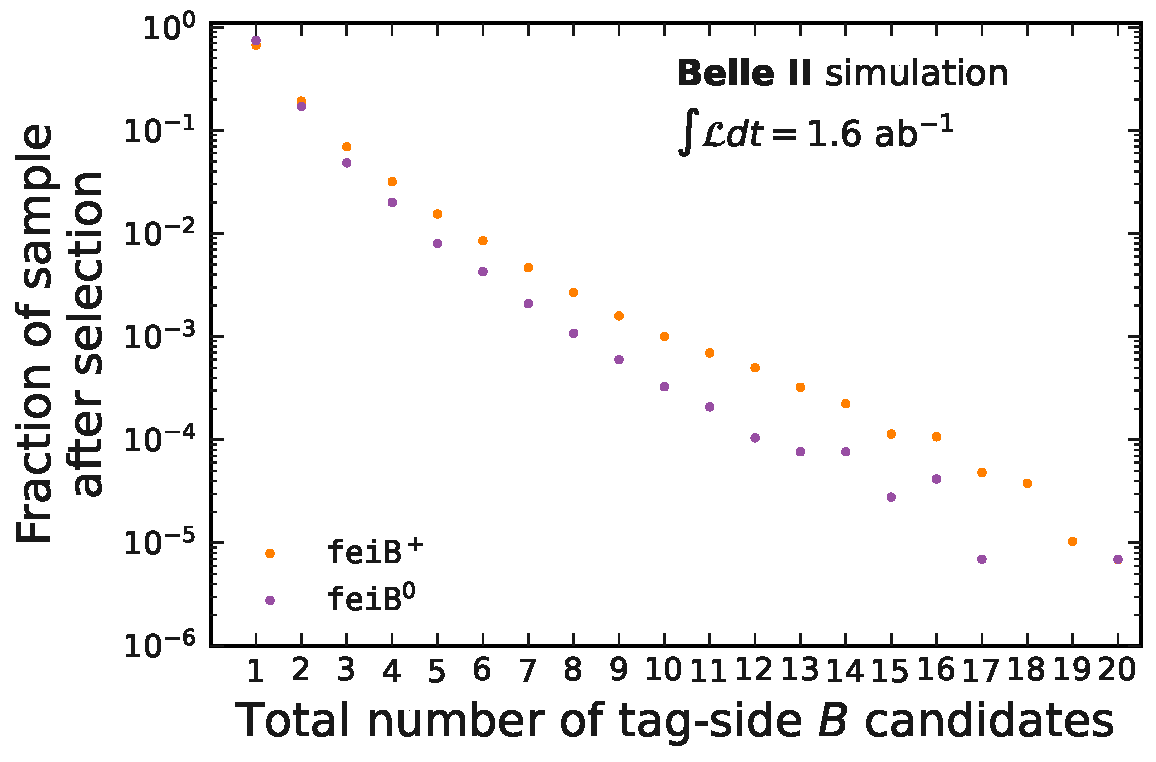
\includegraphics[width=0.45\textwidth]{figures/best_tag_selection/Bboth_total_tag_candidates_post_optimisation.pdf}
    \caption{\label{fig:fei_tag_reco_candidates_post_optimisation} 
    The relative fractions of events for the number of \B meson candidates in the generic \MC data set after the background suppression selections in \Cref{tab:cutflow}.
    This Figure can be directly compared with \Cref{fig:fei_tag_reco_candidates}.
    The overall fractions are similar, confirming a valid background suppression procedure which does not introduce a preference towards specific tag-side modes.
    }
\end{figure}

However, even after all selections there often exists more than one \B meson + photon combination.
The first step of the selection of best tag-$B$ is choosing one candidate each in \feiBp and \feiBz modes.
While a general approach could be developed, it was observed that at this stage a particular choice of the tag does not influence the resolution or the average value of the spectrum strongly.
This is visualised in \Cref{fig:same_mode_best_tag_selection}.
For both neutral and charged \BtoXsgamma modes the distributions look similar whether the highest-\feiProb candidate is selected in each event or a random tag-$B$ meson is chosen as the main candidate.
On the other hand, the \Mbc distribution, as expected, has a more distinct peak for the case where the highest \feiProb candidate is picked in each event.
The latter result for \BtoXsgamma is shown in \Cref{fig:same_mbc_best_tag_selection}.
The Figure also includes a similar \Mbc test for the continuum events.

\begin{figure}[hbtp!]
    \centering
    \subcaptionbox{\label{fig:bp_same_mode_best_tag_selection}}{
        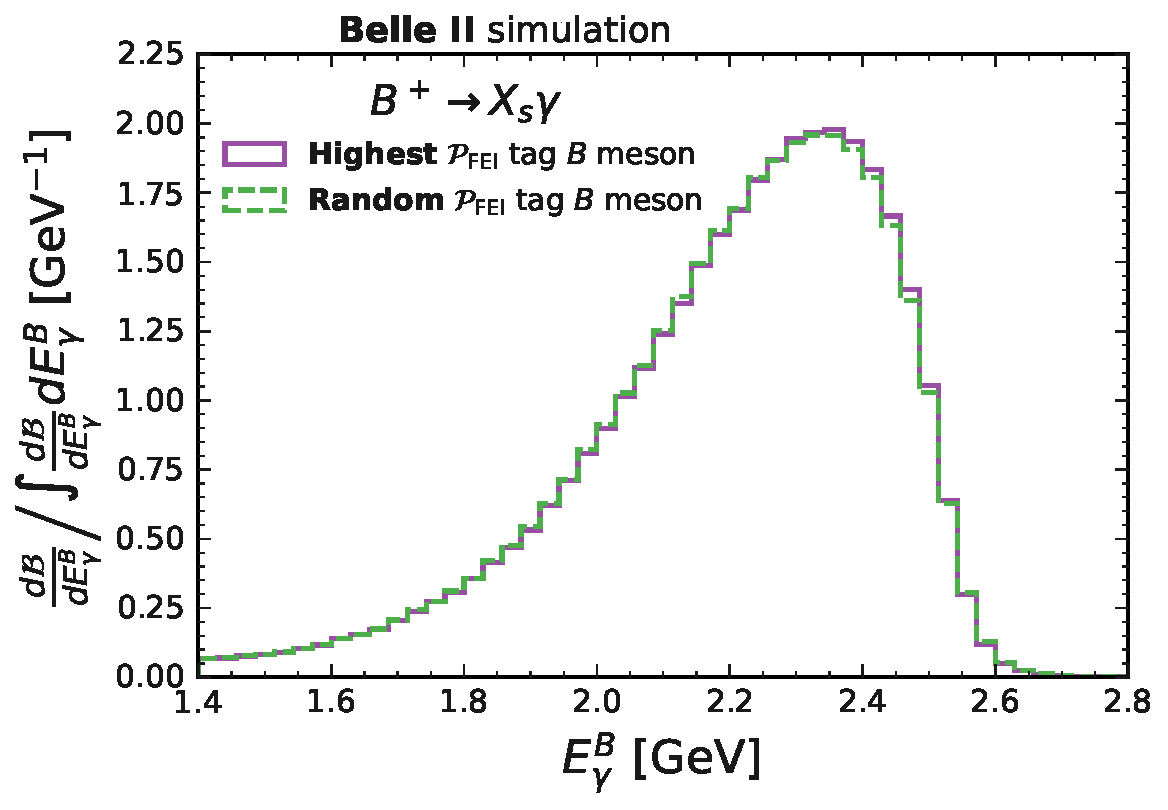
\includegraphics[width=0.4\textwidth]{figures/best_tag_selection/bp_spectrum_with_random_best_tag_selection.pdf}
    }
    \subcaptionbox{\label{fig:bz_same_mode_best_tag_selection}}{
        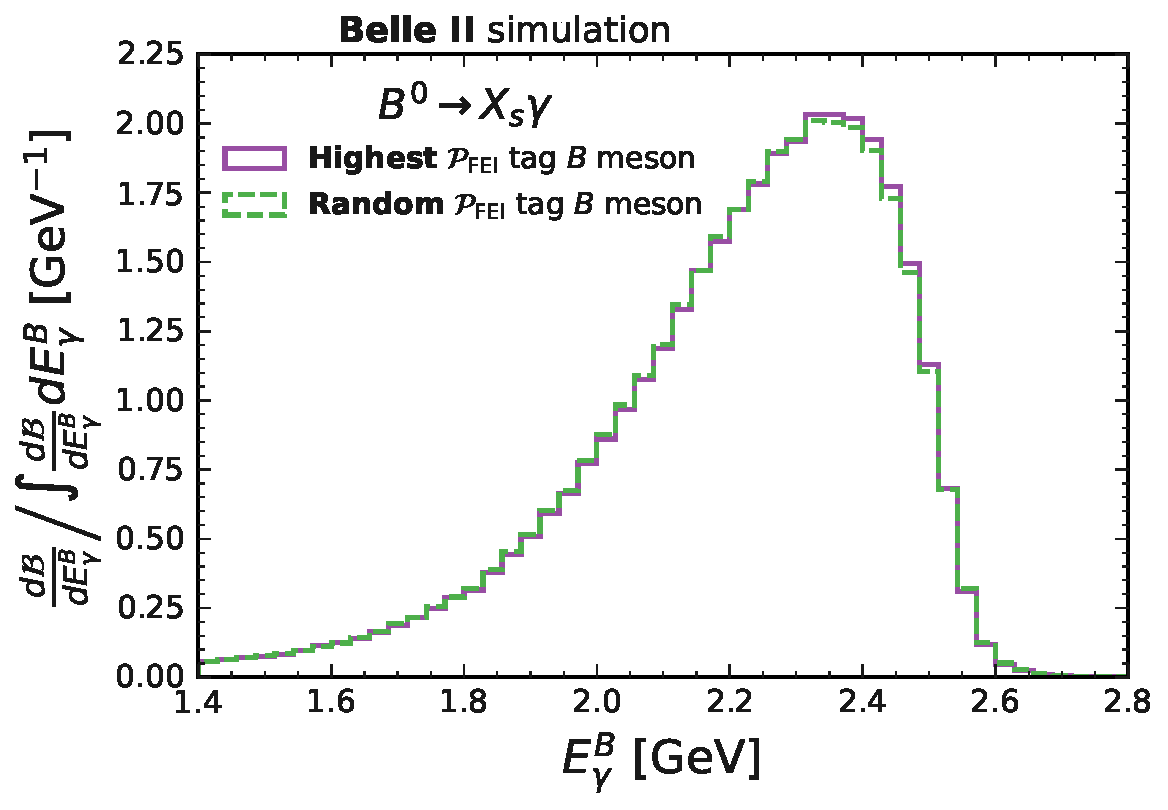
\includegraphics[width=0.4\textwidth]{figures/best_tag_selection/bz_spectrum_with_random_best_tag_selection.pdf}
    }
    \caption{\label{fig:same_mode_best_tag_selection}
    The photon energy spectrum after selecting a single tag-$B$ meson candidate per event either randomly or by requiring the largest \feiProb.
    This is shown for \BptoXsgamma events in (\subref{fig:bp_same_mode_best_tag_selection}) 
    and for \BztoXsgamma in (\subref{fig:bz_same_mode_best_tag_selection}).
    The Figures are normalised to their total integral value such that a shape comparison can be performed.
    The difference between the distributions is negligible.
    }
\end{figure}

\begin{figure}[hbtp!]
    \centering
    \subcaptionbox{\label{fig:bp_mbc_mode_best_tag_selection}}{
        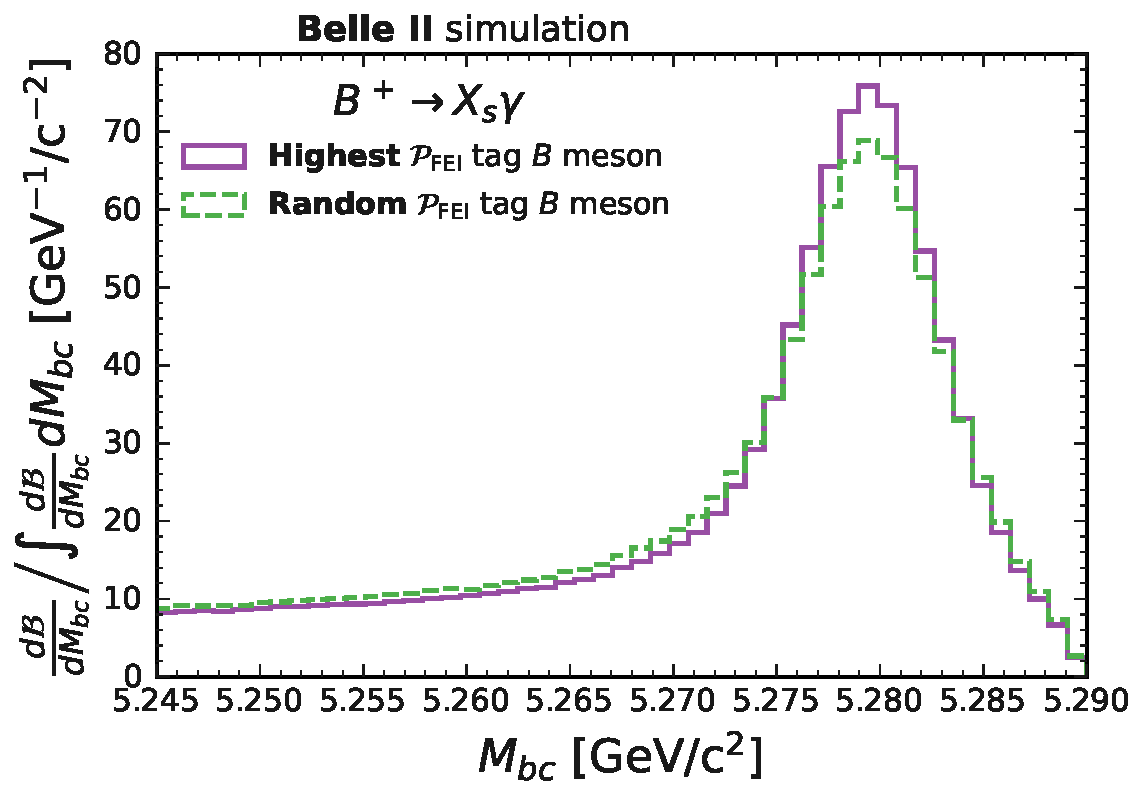
\includegraphics[width=0.45\textwidth]{figures/best_tag_selection/bp_Mbc_with_random_best_tag_selection.pdf}
    }
    \subcaptionbox{\label{fig:bz_mbc_mode_best_tag_selection}}{
        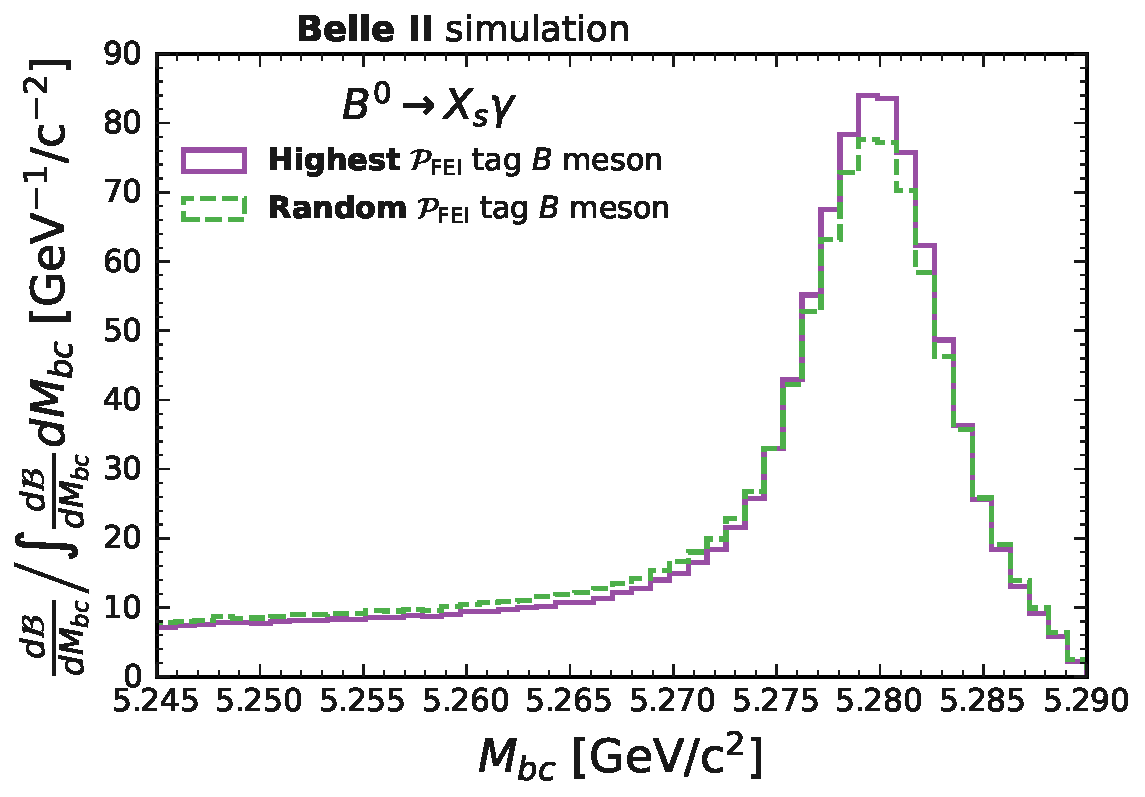
\includegraphics[width=0.45\textwidth]{figures/best_tag_selection/bz_Mbc_with_random_best_tag_selection.pdf}
    }
    \subcaptionbox{\label{fig:bp_continuum_mode_best_tag_selection}}{
        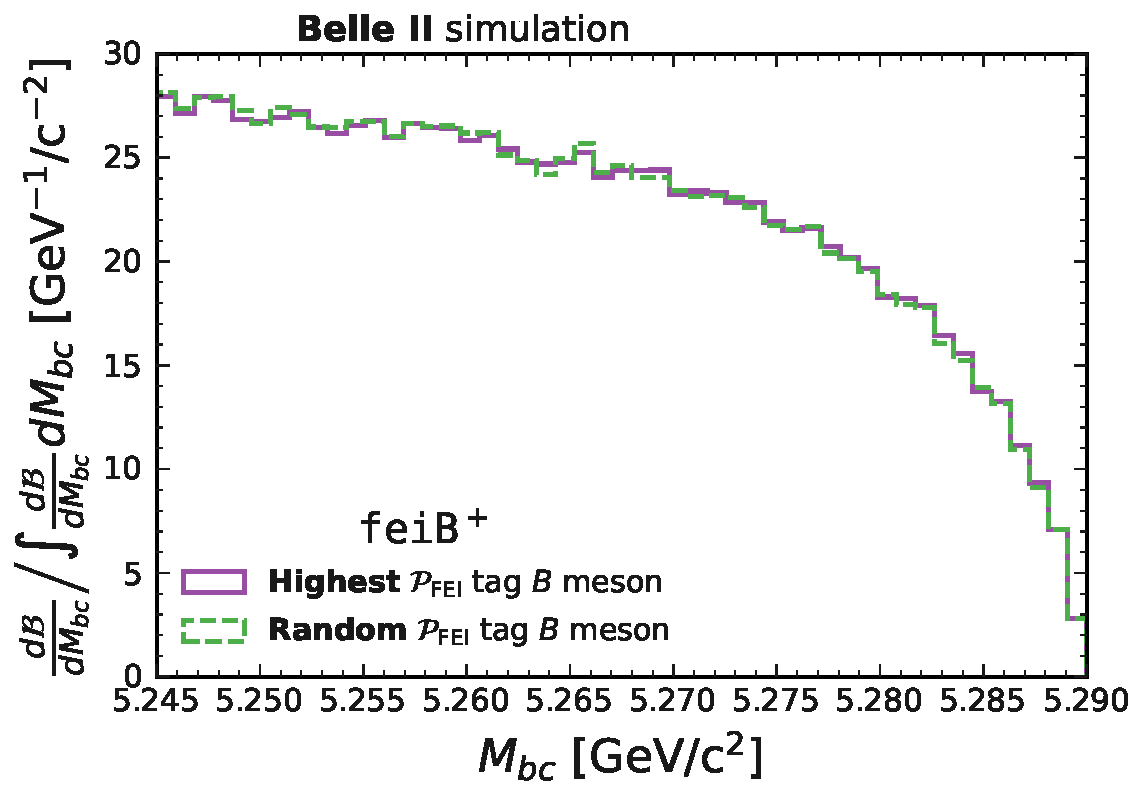
\includegraphics[width=0.45\textwidth]{figures/best_tag_selection/bp_continuum_Mbc_with_random_best_tag_selection.pdf}
    }
    \subcaptionbox{\label{fig:bz_continuum_mode_best_tag_selection}}{
        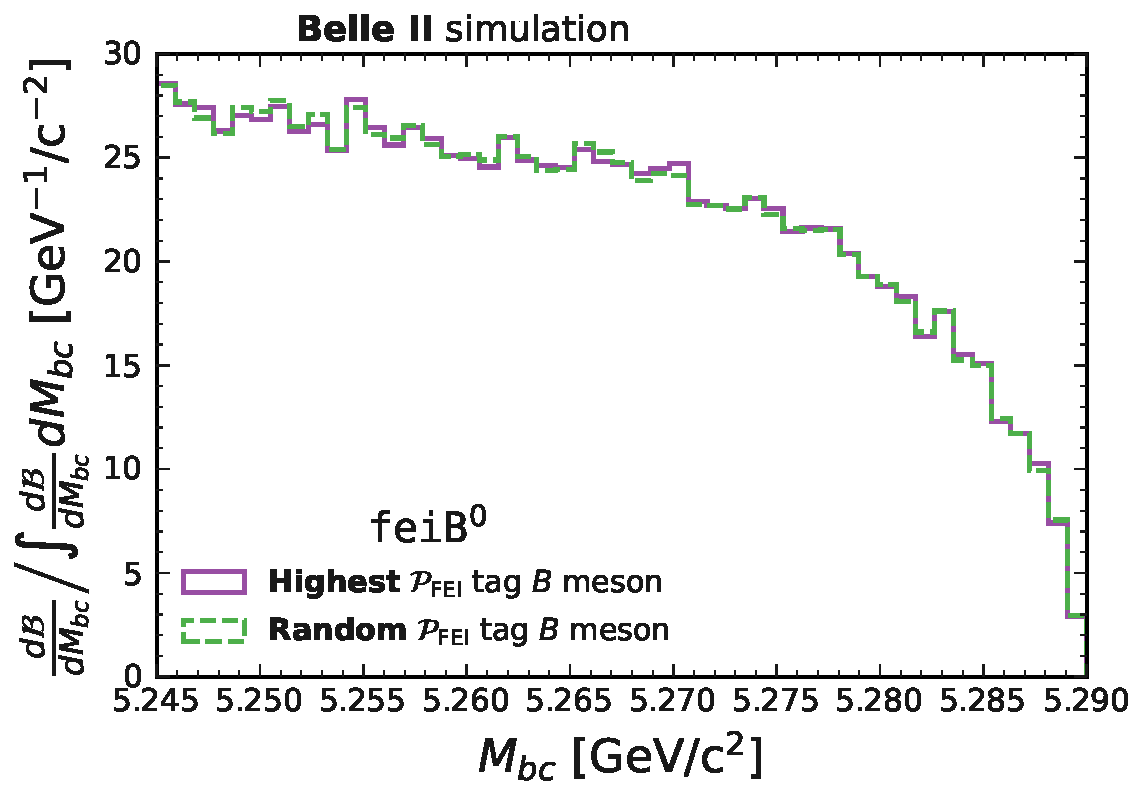
\includegraphics[width=0.45\textwidth]{figures/best_tag_selection/bz_continuum_Mbc_with_random_best_tag_selection.pdf}
    }
    \caption{\label{fig:same_mbc_best_tag_selection}
    The \Mbc shapes for \BtoXsgamma signal \MC ((\subref{fig:bp_mbc_mode_best_tag_selection}) and (\subref{fig:bz_mbc_mode_best_tag_selection})) 
    and \mbox{\epem\ra\qqbar} events from generic \MC ((\subref{fig:bp_continuum_mode_best_tag_selection}) and (\subref{fig:bz_continuum_mode_best_tag_selection})) after selecting a single tag-$B$ meson per event either randomly or by requiring the largest \feiProb.
    As seen in (\subref{fig:bp_mbc_mode_best_tag_selection}) and (\subref{fig:bz_mbc_mode_best_tag_selection}), the difference in the \Mbc distribution for \BptoXsgamma and \BztoXsgamma mostly pronounced in the peak region.
    On the other hand, (\subref{fig:bp_continuum_mode_best_tag_selection}) and (\subref{fig:bz_continuum_mode_best_tag_selection}) show no strong dependence in shape irrespective of the way the tag-side candidate is chosen.
    The Figures are normalised to their total integral value such that a shape comparison can be performed.
    This observation motivates the selection of the highest-\feiProb candidate.
    }    
\end{figure}

As it is desirable to emphasise the contrast between continuum and $B$ events for the fitting step that will follow (see \Cref{sec:fitting_mbc})
the highest \feiProb candidate in each event is chosen as the $B$ candidate with virtually no bias to the resolution.
However, the study here, as of yet, does not address the cases when a candidate in the same event is reconstructed in the \feiBp and \feiBz modes.
Therefore, for now, both candidates are kept in such events and the study is continued in \Cref{sec:select_best_candidate}.

\subsection{Selection between \texorpdfstring{\feiBp}{feiB+} and \texorpdfstring{\feiBz}{feiB0} modes}\label{sec:select_best_candidate}

\Cref{sec:select_tag_between_modes} showed that one can select the highest \feiProb candidate from \feiBp and \feiBz without a significant effect on the \EB resolution and with an enhancement of the \Mbc distribution peak.
It reduced each event to a single tag-$B$ and photon combination in most events.
However, it did not address the case when there is a candidate reconstructed in both \feiBp and \feiBz modes: implying that events may still have up to two combinations.
Such cases are evaluated to happen roughly 10.5\% of the time. 
For the sample where two $B$ candidates exist, two quantities are calculated
\begin{equation}\label{eq:asymmetry_tag}
    \mathcal{A}_{\mathrm{tag}} = \frac{\mathcal{P}_{\mathrm{tag}}(\feiBp) - \mathcal{P}_{\mathrm{tag}}(\feiBz)}{\mathcal{P}_{\mathrm{tag}}(\feiBp) + \mathcal{P}_{\mathrm{tag}}(\feiBz)},
\end{equation}
which is called the asymmetry of \feiProb between a \feiBp and \feiBz candidate in the same event, and
\begin{equation}\label{eq:delta_mbc}
    \Delta(\Mbc) = \Mbc(\Bp) - \Mbc(\Bz),
\end{equation}
which is the difference in \Mbc value of the two candidates.
The $\mathcal{A}_{\mathrm{tag}}$ tends to zero if they both have a similar \feiProb and to $\pm$ unity if one of the candidates has a much larger \feiProb.
The $\Delta(\Mbc)$ is a difference in \Mbc between both of the candidates.
These quantities are visualised in a two-dimensional grid in \Cref{fig:selecting_tag_mode}.
The sample is split into two subsamples, where a real \Bp (\Cref{fig:bp_selecting_tag_mode}) or \Bz (\Cref{fig:bz_selecting_tag_mode}) hadronic decay is present on the tag-side.
If a $\Bp$ candidate is present, $\mathcal{A}_{\mathrm{tag}}\approx1$ and $\Delta(\Mbc)\gtrsim 0$ for the majority of the candidates.
For $\Bz$ candidates the opposite is true: $\mathcal{A}_{\mathrm{tag}}\approx-1$ and $\Delta(\Mbc)\lesssim 0$ for the majority of the candidates.
This result implies that if the true candidate is a \Bp(\Bz), then the value of \feiProb is higher for \feiBp (\feiBz) candidates.
The $\Delta(\Mbc)$ distribution is interpreted by acknowledging that the incorrect candidate is more likely to be present in the \Mbc tail, rather than the peak region.

\begin{figure}[hbtp!]
    \centering
    \subcaptionbox{\label{fig:bp_selecting_tag_mode}}{
        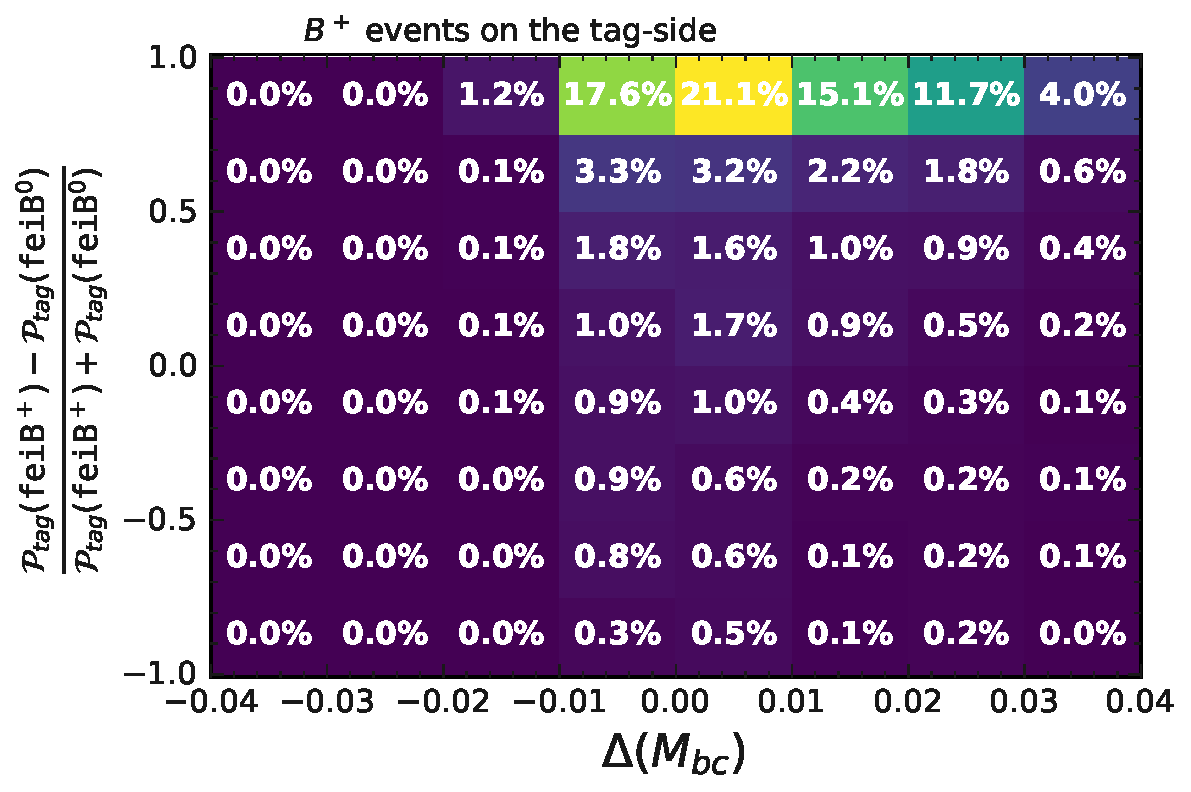
\includegraphics[width=0.45\textwidth]{figures/best_tag_selection/Bp_selecting_between_bp_bz.pdf}
    }
    \subcaptionbox{\label{fig:bz_selecting_tag_mode}}{
        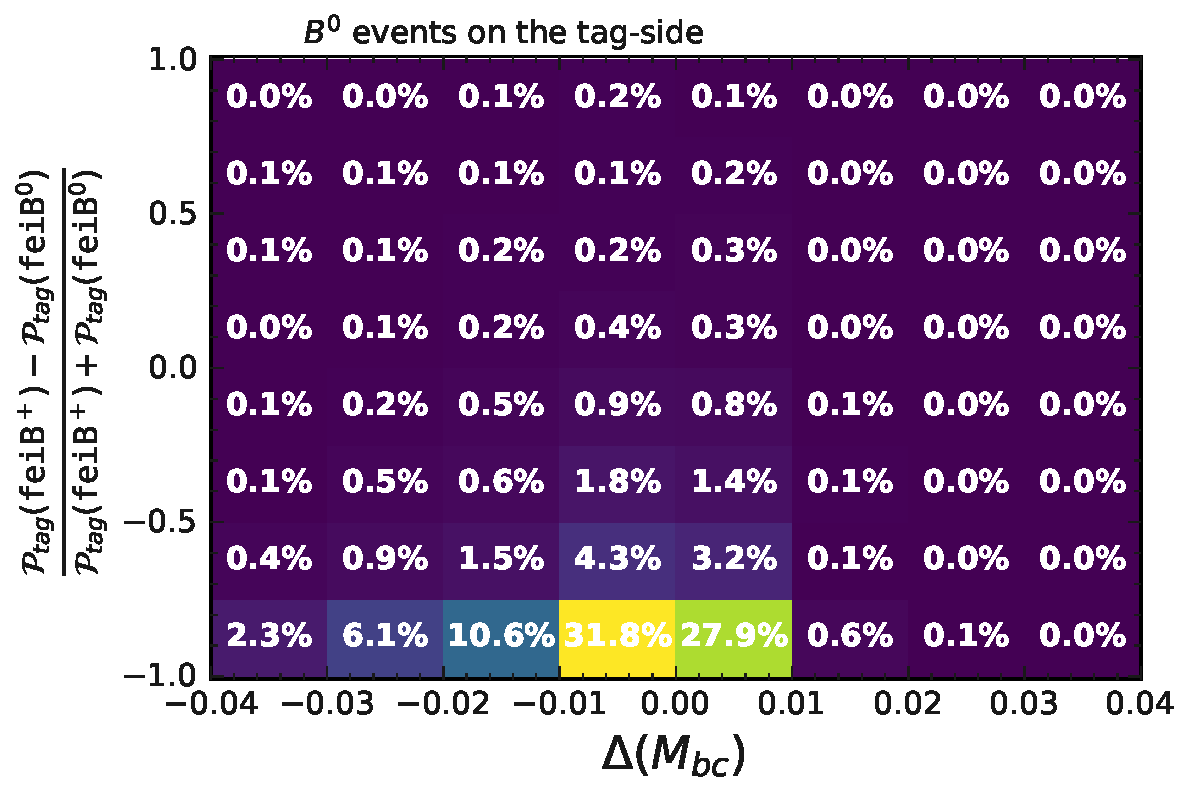
\includegraphics[width=0.45\textwidth]{figures/best_tag_selection/Bz_selecting_between_bp_bz.pdf}
    }
    \caption{\label{fig:selecting_tag_mode} A two-dimensional grid of $\mathcal{A}_{\mathrm{tag}}$ (\Cref{eq:asymmetry_tag})
    and $\Delta(\Mbc)$ (\Cref{eq:delta_mbc}) for events that have two $B$ candidates from \feiBp and \feiBz modes.
    Candidates with a real tag-side $B^+$ decay (\subref{fig:bp_selecting_tag_mode})
    and a real tag-side $B^0$ decay (\subref{fig:bz_selecting_tag_mode}) are shown.
    Most candidates lie near $\mathcal{A}_{\mathrm{tag}}\approx +1 (-1)$ and
    $\Delta(\Mbc)$ value tends to be positive (negative) for $\Bp(\Bz)$ candidates.
    The percentages show the fraction of candidates falling in a two-dimension bin.
    }
\end{figure}

Based on the observations discussed in this Section, it can be concluded that it is appropriate to select the \FEI candidate with the highest signal probability even when selecting between different \feiBp and \feiBz modes.
This result finalises the best-candidate selection in this analysis.
It is now ensured that every photon candidate corresponds to a unique tag-side $B$ meson candidate.

\subsection{Truth-level tag-\texorpdfstring{\B}{B} mesons}\label{sec:good_tag_definition}

In particle physics simulation it is possible to rely on the information provided by the \MC generators to trace back the measured and reconstructed particles to the generated particles.
This procedure is called \textit{truth-matching} and is the usual way to associate `measured objects' and `generated objects'.
In particular, the truth-matching requirements ensure that all the particles have the correct particle species hypotheses, momenta and energies determined.
Furthermore, if unstable, the same should be true for their entire decay chain.
In signal \MC, this allows to study, for example, exclusively the the signal events with successful reconstruction.
However, in the case of tag-$B$ meson reconstruction, it is not particularly important to know that the $B$ meson and its entire decay chain are reconstructed fully correctly.
The most crucial requirement for a tag-$B$ is the consistent kinematic constraint that it can provide to infer the information about the signal-side.
In this analysis, a good kinematic constraint manifests as resonant behaviour in \Mbc for the tag-$B$ meson distribution.

Using \texttt{basf2} truth-level information, the reconstructed tag-$B$ mesons are subdivided into 11 categories based on the differences from the generated decay chains.
The categories are as follows:
\begin{enumerate}
    \setcounter{enumi}{0}
    \item The tag-$B$ and all its daughters are correctly identified and associated;
    \item A final-state radiation photon is not reconstructed;
    \item The tag-$B$ contains more non-final state particles (i.e. resonances) that were not reconstructed;
    \item The tag-$B$ was reconstructed from the secondary decay product which implies that a wrong species hypothesis was used;
    \item The tag-$B$ has a missing neutrino;
    \item The tag-$B$ has a photon missing;
    \item The tag-$B$ has a massive final-state particle missing;
    \item The tag-$B$ has a $K_L^0$ missing (special category compared to 6);
    \item The tag-$B$ has a final state particle associated that has a wrong-signed charge;
    \item The tag-$B$ has a (n-th) daughter non-final-state particle which belongs to a different particle;
    \item Different errors in the truth-matching procedure.
\end{enumerate}
Furthermore, all possible combinations between these are created (e.g. the tag-$B$ has a photon \textit{and} a massive final-state particle missing).
In total, 108 combined categories are observed in the \BtoXsgamma signal \MC samples for $B$ meson candidates.
Most categories, particularly higher-order combinations, do not have any entries in simulated data samples due to their rareness or kinematic inconsistency.

For all tag-$B$ meson candidates in signal \MC within each category, an \Mbc distribution is produced 
and the Jensen-Shannon distance is calculated with respect to category 0 (attributed to perfect reconstruction).
As category 0 (by definition) provides the \textit{best possible kinematic constraint}, the Jensen-Shannon distance is sought to be as close to zero as possible.
Such a result would imply that the difference of the reconstructed tag-$B$ meson is inconsequential to the quality of the constraint.
As an additional metric, for each category, the fraction of $B$ meson candidates with $\Mbc<5.26~\gevcc$ is evaluated.
In a perfect reconstruction case, this number is practically zero.

The two-dimensional distribution of Jensen-Shannon distances and the fraction of $B$ meson candidates with $\Mbc<5.26~\gevcc$
for all 108 combined categories is shown in \Cref{fig:good_tags_jsdists}.
\begin{figure}[hbtp!]
    \centering
    \subcaptionbox{\label{fig:Bp_good_tags_jsdists}}{
        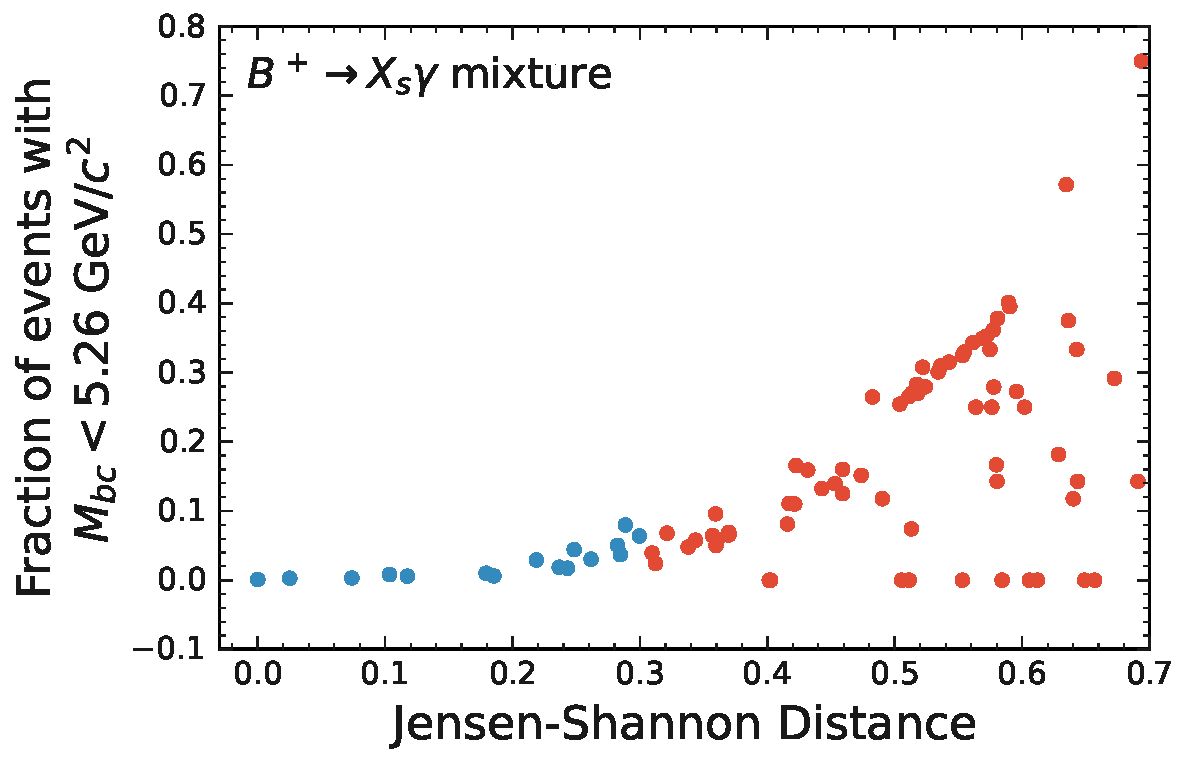
\includegraphics[width=0.31\textwidth]{figures/best_tag_selection/Bp_good_tags_definition.pdf}
    }
    \subcaptionbox{\label{fig:Bz_good_tags_jsdists}}{
        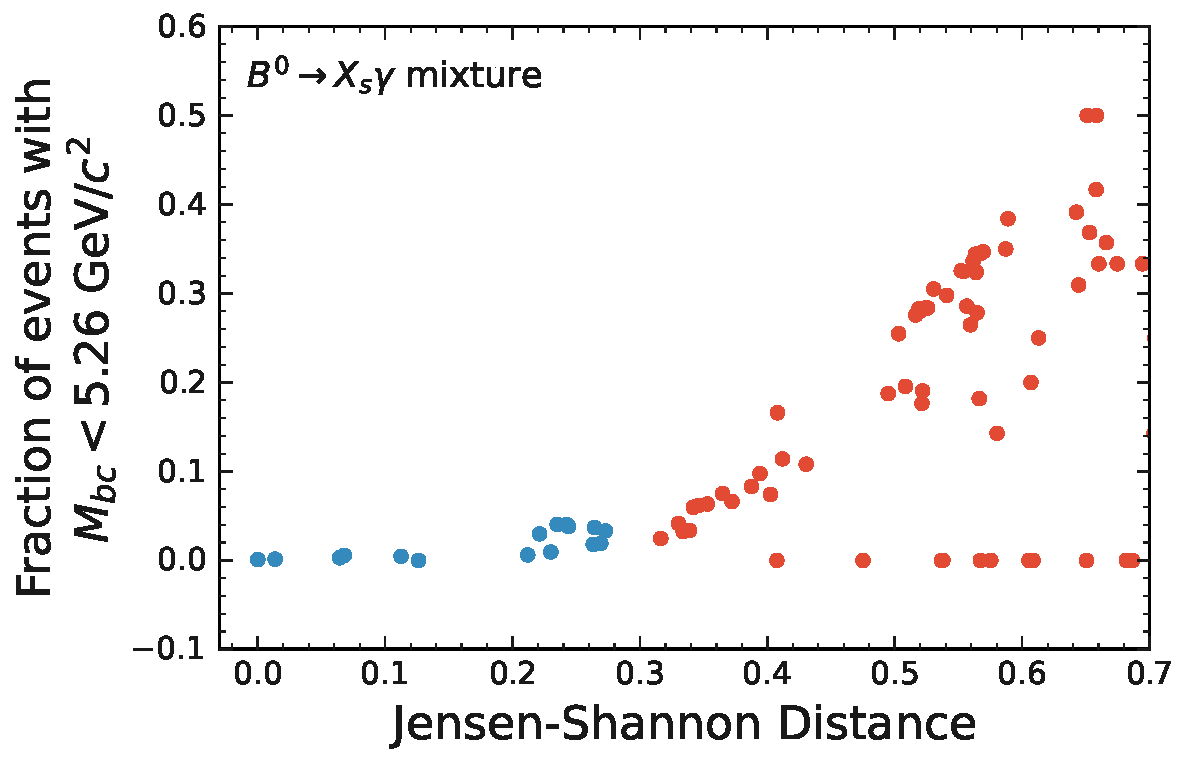
\includegraphics[width=0.31\textwidth]{figures/best_tag_selection/Bz_good_tags_definition.pdf}
    }
    \subcaptionbox{\label{fig:Bboth_good_tags_jsdists}}{
        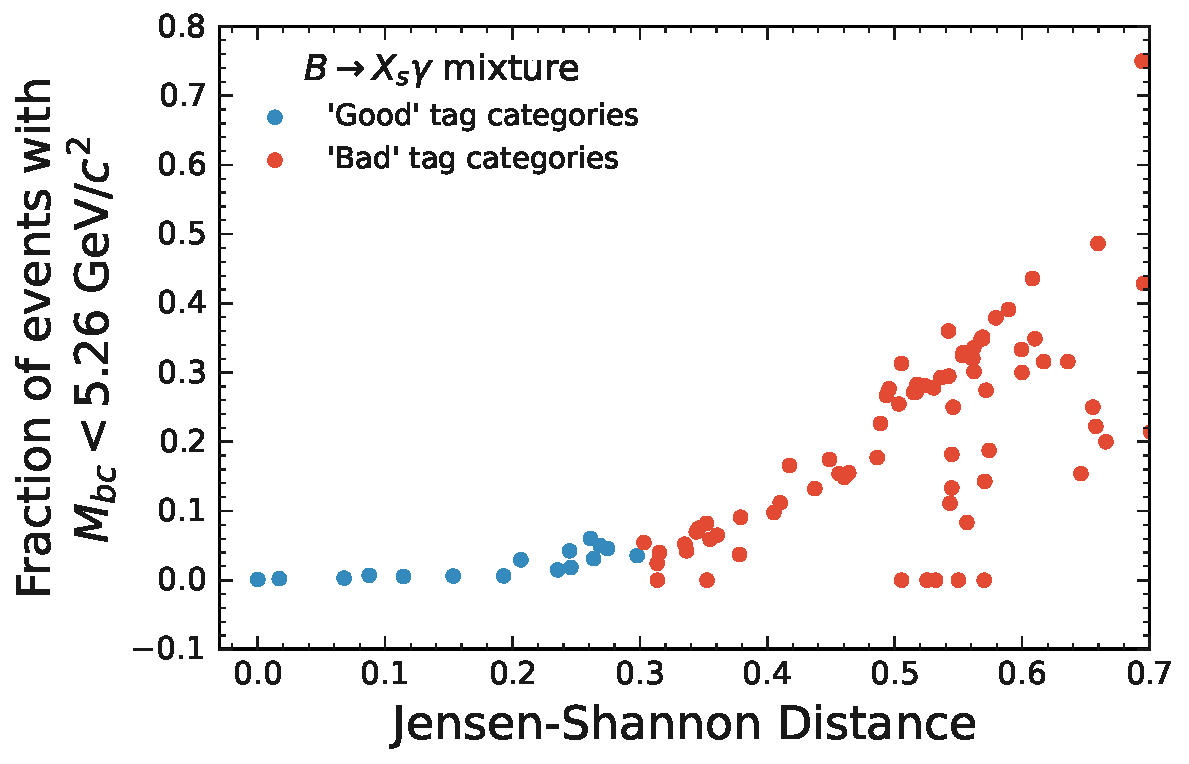
\includegraphics[width=0.31\textwidth]{figures/best_tag_selection/Bboth_good_tags_definition.pdf}
    }
    \caption{\label{fig:good_tags_jsdists} The two-dimensional distribution of Jensen-Shannon distances and the fraction of $B$ meson candidates with $\Mbc<5.26~\gevcc$
    shown for \BptoXsgamma (\subref{fig:Bp_good_tags_jsdists}), \BztoXsgamma (\subref{fig:Bz_good_tags_jsdists}), and the mixture of the two (\subref{fig:Bboth_good_tags_jsdists}).
    108 categories in total have their \Mbc distributions evaluated.
    The legend is shared between the Figures.
    The blue dots are chosen as the definition of tags providing a good kinematic constraint (good tags).
    The choice is based on a threshold of Jensen-Shannon distance $\approx0.3$, where it can be seen that the fraction of $B$ meson candidates with $\Mbc<5.26~\gevcc$ begins to swiftly grow.
    }
\end{figure}
For charged, neutral and mixture of the two samples, the fraction of $B$ meson candidates with $\Mbc<5.26~\gevcc$ begins to swiftly grow at Jensen-Shannon distance $\approx0.3$.
The requirement of Jensen-Shannon distance $<0.3$ is adopted as the threshold to consider a $B$ meson reconstruction category as providing a good kinematic constraint.
The results between different categories are consistent: the same modes are extracted for \Bp, \Bz and the mixture of two.
The categories associated with a good kinematic constraint are summarised in \Cref{tab:error_codes}.
\begin{table}[hbtp!]
    \centering
    \caption{\label{tab:error_codes}Categories of tag-$B$ reconstruction that provide a good kinematic constraint.
    These categories correspond to the blue points in \Cref{fig:Bboth_good_tags_jsdists}.
    The definitions of each category are provided in the text of \Cref{sec:good_tag_definition}.
    }
    \begin{tabular}{c|c}
    \hline
    Category number    & Jensen-Shannon distance  \\ \hline
    1                  & 0          \\ \hline
    9                & 0.02       \\ \hline
    8                & 0.07       \\ \hline
    9,8                & 0.09       \\ \hline
    3                  & 0.11       \\ \hline
    9,3                & 0.15       \\ \hline
    5                 & 0.19       \\ \hline
    8,3                & 0.21       \\ \hline
    5,3                 & 0.24       \\ \hline
    6                 & 0.24       \\ \hline
    8,5,3                & 0.25       \\ \hline
    9,6                & 0.26       \\ \hline
    9,5                & 0.26       \\ \hline
    8,6                & 0.27       \\ \hline
    6,5                 & 0.27       \\ \hline
    9,5,3                & 0.30       \\ \hline
\end{tabular}
\end{table}


The \Mbc distributions for \BtoXsgamma with categories providing a good kinematic constraint and a bad one are shown in \Cref{fig:goodbad_comparison}.
The same Figure also highlights the difference if no procedure such as the one described in this Subsection would be introduced.
One can see a resonant behaviour of imperfectly reconstructed tags in \Cref{fig:isSig_comparison}, which is mostly absorbed into the definition of a good tag provided.
This highlights the importance of the study presented in this Section -- it would be difficult to separate the imperfectly reconstructed tag-$B$ meson distribution from the perfectly reconstructed one in an \Mbc fit that will follow (see \Cref{sec:fitting_mbc}), due to a large correlation between their shapes.
For the rest of this thesis, a tag-$B$ meson that provides a good kinematic constraint will simply be referred to as a \textit{peaking} tag, referencing their behaviour in \Mbc.

\begin{figure}[hbtp!]
    \centering
    \subcaptionbox{\label{fig:goodbad_comparison}}{
        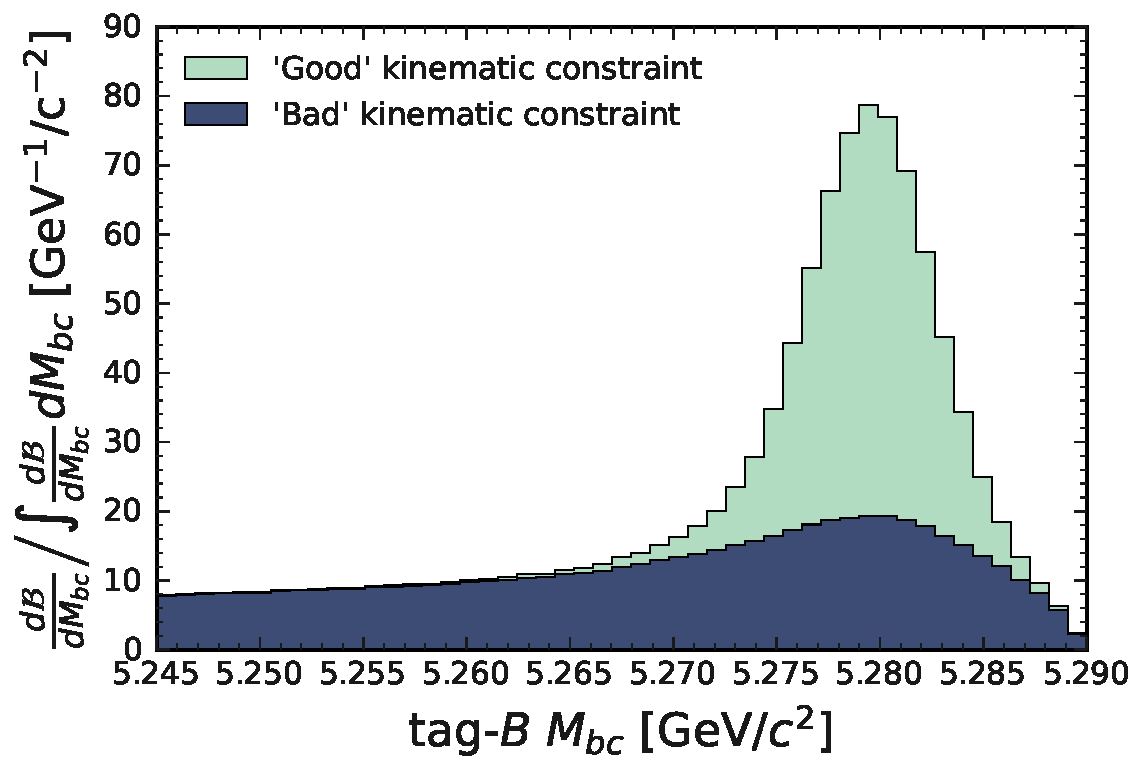
\includegraphics[width=0.4\textwidth]{figures/best_tag_selection/goodbad_tag_comparison.pdf}
    }
    \subcaptionbox{\label{fig:isSig_comparison}}{
        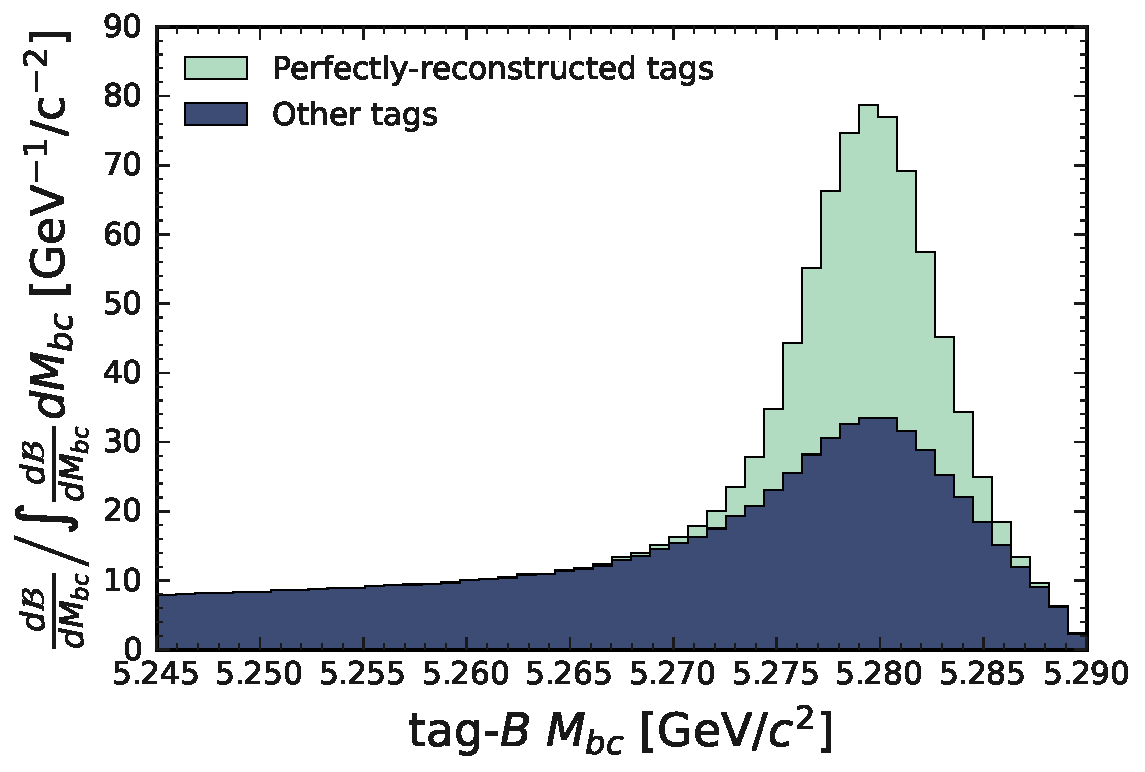
\includegraphics[width=0.4\textwidth]{figures/best_tag_selection/isSig_tag_comparison.pdf}
    }
    \caption{\label{fig:good_tag_definitions} \Mbc distributions of \BtoXsgamma split by good/bad kinematic constraint criterion (\subref{fig:goodbad_comparison})
    and the conventional perfect/imperfect reconstruction criterion (\subref{fig:isSig_comparison}).
    The definition of the tag-$B$ meson described in \Cref{sec:good_tag_definition}
    accurately represents the resonant \Mbc structure.
    }
\end{figure}